\documentclass[12pt]{article}

\usepackage{xspace}
\usepackage{amsfonts}       % blackboard math symbols
\usepackage{nicefrac}       % compact symbols for 1/2, etc.
\usepackage{booktabs}       % professional-quality tables
\usepackage{placeins}

\usepackage[table,xcdraw]{xcolor}
\usepackage[utf8]{inputenc} % allow utf-8 input
\usepackage[T1]{fontenc}    % use 8-bit T1 fonts
\usepackage{hyperref}       % hyperlinks
\usepackage{url}            % simple URL typesetting
\usepackage{booktabs}       % professional-quality tables
\usepackage{amsfonts}       % blackboard math symbols
\usepackage{nicefrac}       % compact symbols for 1/2, etc.
\usepackage{microtype}      % microtypography
\usepackage{stmaryrd}
\usepackage{todonotes}
\usepackage{dsfont}
\usepackage{makecell}
\usepackage{amsthm}
\usepackage{adjustbox}
% \usepackage[lofdepth,lotdepth]{subfig}

\usepackage{algorithm}
\usepackage{algorithmic}
\usepackage{varwidth}
\usepackage{graphicx}
\usepackage{enumitem}
\usepackage{color}
\usepackage{xspace}
\usepackage{subcaption}
\usepackage{caption} 
\usepackage{array}
\usepackage{multirow}
\usepackage{appendix}
\usepackage{mathtools}


%%%%% NEW MATH DEFINITIONS %%%%%

\usepackage{amsmath,amsfonts,bm}

% Mark sections of captions for referring to divisions of figures
\newcommand{\figleft}{{\em (Left)}}
\newcommand{\figcenter}{{\em (Center)}}
\newcommand{\figright}{{\em (Right)}}
\newcommand{\figtop}{{\em (Top)}}
\newcommand{\figbottom}{{\em (Bottom)}}
\newcommand{\captiona}{{\em (a)}}
\newcommand{\captionb}{{\em (b)}}
\newcommand{\captionc}{{\em (c)}}
\newcommand{\captiond}{{\em (d)}}

% Highlight a newly defined term
\newcommand{\newterm}[1]{{\bf #1}}


% Figure reference, lower-case.
\def\figref#1{figure~\ref{#1}}
% Figure reference, capital. For start of sentence
\def\Figref#1{Figure~\ref{#1}}
\def\twofigref#1#2{figures \ref{#1} and \ref{#2}}
\def\quadfigref#1#2#3#4{figures \ref{#1}, \ref{#2}, \ref{#3} and \ref{#4}}
% Section reference, lower-case.
\def\secref#1{section~\ref{#1}}
% Section reference, capital.
\def\Secref#1{Section~\ref{#1}}
% Reference to two sections.
\def\twosecrefs#1#2{sections \ref{#1} and \ref{#2}}
% Reference to three sections.
\def\secrefs#1#2#3{sections \ref{#1}, \ref{#2} and \ref{#3}}
% Reference to an equation, lower-case.
%\def\eqref#1{equation~\ref{#1}}
% Reference to an equation, upper case
%\def\Eqref#1{Equation~\ref{#1}}
% A raw reference to an equation---avoid using if possible
\def\plaineqref#1{\ref{#1}}
% Reference to a chapter, lower-case.
\def\chapref#1{chapter~\ref{#1}}
% Reference to an equation, upper case.
\def\Chapref#1{Chapter~\ref{#1}}
% Reference to a range of chapters
\def\rangechapref#1#2{chapters\ref{#1}--\ref{#2}}
% Reference to an algorithm, lower-case.
\def\algref#1{algorithm~\ref{#1}}
% Reference to an algorithm, upper case.
\def\Algref#1{Algorithm~\ref{#1}}
\def\twoalgref#1#2{algorithms \ref{#1} and \ref{#2}}
\def\Twoalgref#1#2{Algorithms \ref{#1} and \ref{#2}}
% Reference to a part, lower case
\def\partref#1{part~\ref{#1}}
% Reference to a part, upper case
\def\Partref#1{Part~\ref{#1}}
\def\twopartref#1#2{parts \ref{#1} and \ref{#2}}

\def\ceil#1{\lceil #1 \rceil}
\def\floor#1{\lfloor #1 \rfloor}
\def\1{\bm{1}}
\newcommand{\train}{\mathcal{D}}
\newcommand{\valid}{\mathcal{D_{\mathrm{valid}}}}
\newcommand{\test}{\mathcal{D_{\mathrm{test}}}}

\def\eps{{\epsilon}}


% Random variables
\def\reta{{\textnormal{$\eta$}}}
\def\ra{{\textnormal{a}}}
\def\rb{{\textnormal{b}}}
\def\rc{{\textnormal{c}}}
\def\rd{{\textnormal{d}}}
\def\re{{\textnormal{e}}}
\def\rf{{\textnormal{f}}}
\def\rg{{\textnormal{g}}}
\def\rh{{\textnormal{h}}}
\def\ri{{\textnormal{i}}}
\def\rj{{\textnormal{j}}}
\def\rk{{\textnormal{k}}}
\def\rl{{\textnormal{l}}}
% rm is already a command, just don't name any random variables m
\def\rn{{\textnormal{n}}}
\def\ro{{\textnormal{o}}}
\def\rp{{\textnormal{p}}}
\def\rq{{\textnormal{q}}}
\def\rr{{\textnormal{r}}}
\def\rs{{\textnormal{s}}}
\def\rt{{\textnormal{t}}}
\def\ru{{\textnormal{u}}}
\def\rv{{\textnormal{v}}}
\def\rw{{\textnormal{w}}}
\def\rx{{\textnormal{x}}}
\def\ry{{\textnormal{y}}}
\def\rz{{\textnormal{z}}}

% Random vectors
\def\rvepsilon{{\mathbf{\epsilon}}}
\def\rvtheta{{\mathbf{\theta}}}
\def\rva{{\mathbf{a}}}
\def\rvb{{\mathbf{b}}}
\def\rvc{{\mathbf{c}}}
\def\rvd{{\mathbf{d}}}
\def\rve{{\mathbf{e}}}
\def\rvf{{\mathbf{f}}}
\def\rvg{{\mathbf{g}}}
\def\rvh{{\mathbf{h}}}
\def\rvu{{\mathbf{i}}}
\def\rvj{{\mathbf{j}}}
\def\rvk{{\mathbf{k}}}
\def\rvl{{\mathbf{l}}}
\def\rvm{{\mathbf{m}}}
\def\rvn{{\mathbf{n}}}
\def\rvo{{\mathbf{o}}}
\def\rvp{{\mathbf{p}}}
\def\rvq{{\mathbf{q}}}
\def\rvr{{\mathbf{r}}}
\def\rvs{{\mathbf{s}}}
\def\rvt{{\mathbf{t}}}
\def\rvu{{\mathbf{u}}}
\def\rvv{{\mathbf{v}}}
\def\rvw{{\mathbf{w}}}
\def\rvx{{\mathbf{x}}}
\def\rvy{{\mathbf{y}}}
\def\rvz{{\mathbf{z}}}

% Elements of random vectors
\def\erva{{\textnormal{a}}}
\def\ervb{{\textnormal{b}}}
\def\ervc{{\textnormal{c}}}
\def\ervd{{\textnormal{d}}}
\def\erve{{\textnormal{e}}}
\def\ervf{{\textnormal{f}}}
\def\ervg{{\textnormal{g}}}
\def\ervh{{\textnormal{h}}}
\def\ervi{{\textnormal{i}}}
\def\ervj{{\textnormal{j}}}
\def\ervk{{\textnormal{k}}}
\def\ervl{{\textnormal{l}}}
\def\ervm{{\textnormal{m}}}
\def\ervn{{\textnormal{n}}}
\def\ervo{{\textnormal{o}}}
\def\ervp{{\textnormal{p}}}
\def\ervq{{\textnormal{q}}}
\def\ervr{{\textnormal{r}}}
\def\ervs{{\textnormal{s}}}
\def\ervt{{\textnormal{t}}}
\def\ervu{{\textnormal{u}}}
\def\ervv{{\textnormal{v}}}
\def\ervw{{\textnormal{w}}}
\def\ervx{{\textnormal{x}}}
\def\ervy{{\textnormal{y}}}
\def\ervz{{\textnormal{z}}}

% Random matrices
\def\rmA{{\mathbf{A}}}
\def\rmB{{\mathbf{B}}}
\def\rmC{{\mathbf{C}}}
\def\rmD{{\mathbf{D}}}
\def\rmE{{\mathbf{E}}}
\def\rmF{{\mathbf{F}}}
\def\rmG{{\mathbf{G}}}
\def\rmH{{\mathbf{H}}}
\def\rmI{{\mathbf{I}}}
\def\rmJ{{\mathbf{J}}}
\def\rmK{{\mathbf{K}}}
\def\rmL{{\mathbf{L}}}
\def\rmM{{\mathbf{M}}}
\def\rmN{{\mathbf{N}}}
\def\rmO{{\mathbf{O}}}
\def\rmP{{\mathbf{P}}}
\def\rmQ{{\mathbf{Q}}}
\def\rmR{{\mathbf{R}}}
\def\rmS{{\mathbf{S}}}
\def\rmT{{\mathbf{T}}}
\def\rmU{{\mathbf{U}}}
\def\rmV{{\mathbf{V}}}
\def\rmW{{\mathbf{W}}}
\def\rmX{{\mathbf{X}}}
\def\rmY{{\mathbf{Y}}}
\def\rmZ{{\mathbf{Z}}}

% Elements of random matrices
\def\ermA{{\textnormal{A}}}
\def\ermB{{\textnormal{B}}}
\def\ermC{{\textnormal{C}}}
\def\ermD{{\textnormal{D}}}
\def\ermE{{\textnormal{E}}}
\def\ermF{{\textnormal{F}}}
\def\ermG{{\textnormal{G}}}
\def\ermH{{\textnormal{H}}}
\def\ermI{{\textnormal{I}}}
\def\ermJ{{\textnormal{J}}}
\def\ermK{{\textnormal{K}}}
\def\ermL{{\textnormal{L}}}
\def\ermM{{\textnormal{M}}}
\def\ermN{{\textnormal{N}}}
\def\ermO{{\textnormal{O}}}
\def\ermP{{\textnormal{P}}}
\def\ermQ{{\textnormal{Q}}}
\def\ermR{{\textnormal{R}}}
\def\ermS{{\textnormal{S}}}
\def\ermT{{\textnormal{T}}}
\def\ermU{{\textnormal{U}}}
\def\ermV{{\textnormal{V}}}
\def\ermW{{\textnormal{W}}}
\def\ermX{{\textnormal{X}}}
\def\ermY{{\textnormal{Y}}}
\def\ermZ{{\textnormal{Z}}}

% Vectors
\def\vzero{{\bm{0}}}
\def\vone{{\bm{1}}}
\def\vmu{{\bm{\mu}}}
\def\vtheta{{\bm{\theta}}}
\def\va{{\bm{a}}}
\def\vb{{\bm{b}}}
\def\vc{{\bm{c}}}
\def\vd{{\bm{d}}}
\def\ve{{\bm{e}}}
\def\vf{{\bm{f}}}
\def\vg{{\bm{g}}}
\def\vh{{\bm{h}}}
\def\vi{{\bm{i}}}
\def\vj{{\bm{j}}}
\def\vk{{\bm{k}}}
\def\vl{{\bm{l}}}
\def\vm{{\bm{m}}}
\def\vn{{\bm{n}}}
\def\vo{{\bm{o}}}
\def\vp{{\bm{p}}}
\def\vq{{\bm{q}}}
\def\vr{{\bm{r}}}
\def\vs{{\bm{s}}}
\def\vt{{\bm{t}}}
\def\vu{{\bm{u}}}
\def\vv{{\bm{v}}}
\def\vw{{\bm{w}}}
\def\vx{{\bm{x}}}
\def\vy{{\bm{y}}}
\def\vz{{\bm{z}}}

% Elements of vectors
\def\evalpha{{\alpha}}
\def\evbeta{{\beta}}
\def\evepsilon{{\epsilon}}
\def\evlambda{{\lambda}}
\def\evomega{{\omega}}
\def\evmu{{\mu}}
\def\evpsi{{\psi}}
\def\evsigma{{\sigma}}
\def\evtheta{{\theta}}
\def\eva{{a}}
\def\evb{{b}}
\def\evc{{c}}
\def\evd{{d}}
\def\eve{{e}}
\def\evf{{f}}
\def\evg{{g}}
\def\evh{{h}}
\def\evi{{i}}
\def\evj{{j}}
\def\evk{{k}}
\def\evl{{l}}
\def\evm{{m}}
\def\evn{{n}}
\def\evo{{o}}
\def\evp{{p}}
\def\evq{{q}}
\def\evr{{r}}
\def\evs{{s}}
\def\evt{{t}}
\def\evu{{u}}
\def\evv{{v}}
\def\evw{{w}}
\def\evx{{x}}
\def\evy{{y}}
\def\evz{{z}}

% Matrix
\def\mA{{\bm{A}}}
\def\mB{{\bm{B}}}
\def\mC{{\bm{C}}}
\def\mD{{\bm{D}}}
\def\mE{{\bm{E}}}
\def\mF{{\bm{F}}}
\def\mG{{\bm{G}}}
\def\mH{{\bm{H}}}
\def\mI{{\bm{I}}}
\def\mJ{{\bm{J}}}
\def\mK{{\bm{K}}}
\def\mL{{\bm{L}}}
\def\mM{{\bm{M}}}
\def\mN{{\bm{N}}}
\def\mO{{\bm{O}}}
\def\mP{{\bm{P}}}
\def\mQ{{\bm{Q}}}
\def\mR{{\bm{R}}}
\def\mS{{\bm{S}}}
\def\mT{{\bm{T}}}
\def\mU{{\bm{U}}}
\def\mV{{\bm{V}}}
\def\mW{{\bm{W}}}
\def\mX{{\bm{X}}}
\def\mY{{\bm{Y}}}
\def\mZ{{\bm{Z}}}
\def\mBeta{{\bm{\beta}}}
\def\mPhi{{\bm{\Phi}}}
\def\mLambda{{\bm{\Lambda}}}
\def\mSigma{{\bm{\Sigma}}}

% Tensor
\DeclareMathAlphabet{\mathsfit}{\encodingdefault}{\sfdefault}{m}{sl}
\SetMathAlphabet{\mathsfit}{bold}{\encodingdefault}{\sfdefault}{bx}{n}
\newcommand{\tens}[1]{\bm{\mathsfit{#1}}}
\def\tA{{\tens{A}}}
\def\tB{{\tens{B}}}
\def\tC{{\tens{C}}}
\def\tD{{\tens{D}}}
\def\tE{{\tens{E}}}
\def\tF{{\tens{F}}}
\def\tG{{\tens{G}}}
\def\tH{{\tens{H}}}
\def\tI{{\tens{I}}}
\def\tJ{{\tens{J}}}
\def\tK{{\tens{K}}}
\def\tL{{\tens{L}}}
\def\tM{{\tens{M}}}
\def\tN{{\tens{N}}}
\def\tO{{\tens{O}}}
\def\tP{{\tens{P}}}
\def\tQ{{\tens{Q}}}
\def\tR{{\tens{R}}}
\def\tS{{\tens{S}}}
\def\tT{{\tens{T}}}
\def\tU{{\tens{U}}}
\def\tV{{\tens{V}}}
\def\tW{{\tens{W}}}
\def\tX{{\tens{X}}}
\def\tY{{\tens{Y}}}
\def\tZ{{\tens{Z}}}


% Graph
\def\gA{{\mathcal{A}}}
\def\gB{{\mathcal{B}}}
\def\gC{{\mathcal{C}}}
\def\gD{{\mathcal{D}}}
\def\gE{{\mathcal{E}}}
\def\gF{{\mathcal{F}}}
\def\gG{{\mathcal{G}}}
\def\gH{{\mathcal{H}}}
\def\gI{{\mathcal{I}}}
\def\gJ{{\mathcal{J}}}
\def\gK{{\mathcal{K}}}
\def\gL{{\mathcal{L}}}
\def\gM{{\mathcal{M}}}
\def\gN{{\mathcal{N}}}
\def\gO{{\mathcal{O}}}
\def\gP{{\mathcal{P}}}
\def\gQ{{\mathcal{Q}}}
\def\gR{{\mathcal{R}}}
\def\gS{{\mathcal{S}}}
\def\gT{{\mathcal{T}}}
\def\gU{{\mathcal{U}}}
\def\gV{{\mathcal{V}}}
\def\gW{{\mathcal{W}}}
\def\gX{{\mathcal{X}}}
\def\gY{{\mathcal{Y}}}
\def\gZ{{\mathcal{Z}}}

% Sets
\def\sA{{\mathbb{A}}}
\def\sB{{\mathbb{B}}}
\def\sC{{\mathbb{C}}}
\def\sD{{\mathbb{D}}}
% Don't use a set called E, because this would be the same as our symbol
% for expectation.
\def\sF{{\mathbb{F}}}
\def\sG{{\mathbb{G}}}
\def\sH{{\mathbb{H}}}
\def\sI{{\mathbb{I}}}
\def\sJ{{\mathbb{J}}}
\def\sK{{\mathbb{K}}}
\def\sL{{\mathbb{L}}}
\def\sM{{\mathbb{M}}}
\def\sN{{\mathbb{N}}}
\def\sO{{\mathbb{O}}}
\def\sP{{\mathbb{P}}}
\def\sQ{{\mathbb{Q}}}
\def\sR{{\mathbb{R}}}
\def\sS{{\mathbb{S}}}
\def\sT{{\mathbb{T}}}
\def\sU{{\mathbb{U}}}
\def\sV{{\mathbb{V}}}
\def\sW{{\mathbb{W}}}
\def\sX{{\mathbb{X}}}
\def\sY{{\mathbb{Y}}}
\def\sZ{{\mathbb{Z}}}

% Entries of a matrix
\def\emLambda{{\Lambda}}
\def\emA{{A}}
\def\emB{{B}}
\def\emC{{C}}
\def\emD{{D}}
\def\emE{{E}}
\def\emF{{F}}
\def\emG{{G}}
\def\emH{{H}}
\def\emI{{I}}
\def\emJ{{J}}
\def\emK{{K}}
\def\emL{{L}}
\def\emM{{M}}
\def\emN{{N}}
\def\emO{{O}}
\def\emP{{P}}
\def\emQ{{Q}}
\def\emR{{R}}
\def\emS{{S}}
\def\emT{{T}}
\def\emU{{U}}
\def\emV{{V}}
\def\emW{{W}}
\def\emX{{X}}
\def\emY{{Y}}
\def\emZ{{Z}}
\def\emSigma{{\Sigma}}

% entries of a tensor
% Same font as tensor, without \bm wrapper
\newcommand{\etens}[1]{\mathsfit{#1}}
\def\etLambda{{\etens{\Lambda}}}
\def\etA{{\etens{A}}}
\def\etB{{\etens{B}}}
\def\etC{{\etens{C}}}
\def\etD{{\etens{D}}}
\def\etE{{\etens{E}}}
\def\etF{{\etens{F}}}
\def\etG{{\etens{G}}}
\def\etH{{\etens{H}}}
\def\etI{{\etens{I}}}
\def\etJ{{\etens{J}}}
\def\etK{{\etens{K}}}
\def\etL{{\etens{L}}}
\def\etM{{\etens{M}}}
\def\etN{{\etens{N}}}
\def\etO{{\etens{O}}}
\def\etP{{\etens{P}}}
\def\etQ{{\etens{Q}}}
\def\etR{{\etens{R}}}
\def\etS{{\etens{S}}}
\def\etT{{\etens{T}}}
\def\etU{{\etens{U}}}
\def\etV{{\etens{V}}}
\def\etW{{\etens{W}}}
\def\etX{{\etens{X}}}
\def\etY{{\etens{Y}}}
\def\etZ{{\etens{Z}}}

% The true underlying data generating distribution
\newcommand{\pdata}{p_{\rm{data}}}
% The empirical distribution defined by the training set
\newcommand{\ptrain}{\hat{p}_{\rm{data}}}
\newcommand{\Ptrain}{\hat{P}_{\rm{data}}}
% The model distribution
\newcommand{\pmodel}{p_{\rm{model}}}
\newcommand{\Pmodel}{P_{\rm{model}}}
\newcommand{\ptildemodel}{\tilde{p}_{\rm{model}}}
% Stochastic autoencoder distributions
\newcommand{\pencode}{p_{\rm{encoder}}}
\newcommand{\pdecode}{p_{\rm{decoder}}}
\newcommand{\precons}{p_{\rm{reconstruct}}}

\newcommand{\laplace}{\mathrm{Laplace}} % Laplace distribution

\newcommand{\E}{\mathbb{E}}
\newcommand{\Ls}{\mathcal{L}}
\newcommand{\R}{\mathbb{R}}
\newcommand{\emp}{\tilde{p}}
\newcommand{\lr}{\alpha}
\newcommand{\reg}{\lambda}
\newcommand{\rect}{\mathrm{rectifier}}
\newcommand{\softmax}{\mathrm{softmax}}
\newcommand{\sigmoid}{\sigma}
\newcommand{\softplus}{\zeta}
\newcommand{\KL}{D_{\mathrm{KL}}}
\newcommand{\Var}{\mathrm{Var}}
\newcommand{\standarderror}{\mathrm{SE}}
\newcommand{\Cov}{\mathrm{Cov}}
% Wolfram Mathworld says $L^2$ is for function spaces and $\ell^2$ is for vectors
% But then they seem to use $L^2$ for vectors throughout the site, and so does
% wikipedia.
\newcommand{\normlzero}{L^0}
\newcommand{\normlone}{L^1}
\newcommand{\normltwo}{L^2}
\newcommand{\normlp}{L^p}
\newcommand{\normmax}{L^\infty}

\newcommand{\parents}{Pa} % See usage in notation.tex. Chosen to match Daphne's book.

\DeclareMathOperator*{\argmax}{arg\,max}
\DeclareMathOperator*{\argmin}{arg\,min}

\DeclareMathOperator{\sign}{sign}
\DeclareMathOperator{\Tr}{Tr}
\let\ab\allowbreak

\newcommand{\intint}[1]{\left \llbracket#1\right \rrbracket}



\def\palm{\texttt{palm4MSA}\xspace}
\def\hpalm{\texttt{Hierarchical-palm4MSA}\xspace}
\newcommand{\bigO}[1]{\mathcal{O}\left(#1\right)}
\def\datadim{D}
\def\nexamples{N}
\def\nfactors{Q}

\title{Expressing Neural Network layers as Fast-Transforms}
\author{
        Luc Giffon \\
        QARMA team - LIS\\
        Aix-Marseille Universit\'e\\
        Marseille, France
}
\date{\today}

\begin{document}
\maketitle


\begin{abstract}
We apply the \palm algorithm on a pretrained neural network in order to express the fully-connected weights matrices and the matrix of convolutional filters as fast-transforms. This allows a drastic reduction of the number of parameters in the network and the associated speed-up in computation at inference time when deployed on a single-threaded architecture. This post-training modification of neural networks doesn't impair accuracy performance (or we hope so).

\textbf{Motivation}: No GPU needed at inference time? Less RAM needed? Lower carbon footprint?

\end{abstract}

\section{Introduction}
It is widely accepted that neural networks have been a game changer in the race for best classification accuracy on many image classification and natural language processing (NLP) benchmarks. These, not so new anymore, families of models are able to take advantage of the parallelization power of modern GPUs to learn from udge databases and tune millions of parameters to achieve a given task. 

It must be emphasized though that these amazing results come at a price, both economical and ecological. On one hand, recent work~\cite{DBLP:journals/corr/abs-1906-02243} have pointed out that training some NLP models have a significant energy consumption cost that is directly translatable to financial or carbon footprint considerations. On the other hand, the vast majority of power consumption for neural networks is spent for inference and not for training\cite{amazon_inferencepower} \cite{openai_aiandcompute}. Even though computer vision models aren't as demanding in energy than NLP does yet, it is clear that deploying them at large scale, as they are about to be, will bring concerns of the same nature.

These energy consumption concerns are directly related to the number of parameters necessary to achieve such excellent accuracy results. Indeed, it mainly comes from the many multiplications involved in the inner linear transformations at each layer of neural networks. This udge number of parameter brings also the problem of storing some models in GPUs VRAM, making them particularly unhandy to deploy on small devices such as smartphones. Additionaly, such devices doesn't even have embedded GPU, in which case the amount of computation becomes completely untractable for simple CPU hardware.

\todo[inline]{Introduction to be continued.... mais vous avez saisi l'idée}


% %\paragraph{Notations}


%%%%%%%%%%%%%%%%%%%%%%%%%%%%%%%%%%%%%%%%%%%%%%%%%%%%%%%%%%%%
\begin{table}[t]
	\centering
	\begin{footnotesize}
	\begin{tabular}{ll}\\
\toprule
		{\bf Symbol}  & {\bf Meaning}\\
\midrule
$\intint{H}$  & set of integers from $1$ to $H$\\
$\|\cdot\|$ & $L_2$-norm\\
$\|\cdot\|_F$ &    Frobenius norm  \\
$\|\cdot\|_0$ & $L_0$-norm\\
$\|\cdot\|_2$    &    spectral norm  \\
$\rmD_\rvv$ & diagonal matrix with vector $\rvv$ on the diagonal\\                                                
% $N$           & number of data points\\
$D$           & data dimension\\
$H$           & number of layers in a network\\
$Q$           & number of sparse factors\\
$\mathcal{X}_i$ & input space of $f_{i+1}$ and output space of $f_{i}$\\
$\rvx_1,\ldots, \rvx_N $        &    data points\\
$\rmX \in\mathbb{R}^{N\times D}$&    data matrix\\
$\rmS_1, \ldots, \rmS_Q$        &    sparse matrices\\
$\mathcal{E}_1, \ldots, \mathcal{E}_Q$ & sparsity constraint sets\\
$\delta_{\mathcal{E}}$ & 		indicator functions for set $\mathcal{E}$\\
$\floor{\rvx}$ & round $\rvx$ to the flooring integer\\
% $\tau$  & current iteration \\
\bottomrule
	\end{tabular}
	\end{footnotesize}
	\caption{Notation used in this paper.}
	\label{tab:notation}
\end{table}
%\begin{table}[t]
%	\centering
%	\begin{footnotesize}
%	\begin{tabular}{cllcl}\\
%		\cline{1-2}\cline{4-5}\vspace*{1mm}
%		{\bf Symbol}  & {\bf Meaning}                      &  &    {\bf Symbol}          & {\bf Meaning}                    \\ 		\cline{1-2}\cline{4-5}
%		$N$           & number of data points              &  &    $\rvx_1,\ldots, \rvx_N $        &    data points            \\
%		$D$           & data dimension &  &    $\rmX \in\mathbb{R}^{N\times D}$&    data matrix            \\
%		$K$           & number of clusters                 &  &    $\rvu_1,\ldots, \rvu_K $        &    \kmeans centroids        \\
%		$\rvt$        &  cluster assignment vector           &  &    $\rmU\in\mathbb{R}^{K\times D}$ &    \kmeans centroid matrix  \\
%		&                 &  &    $\rvv_1,\ldots, \rvv_K $        &    \qkmeans centroids        \\
%		&          &  &    $\rmV\in\mathbb{R}^{K\times D}$ &    \qkmeans centroid matrix  \\
%		$Q$           & number of sparse factors    &  &    $\rmS_1, \ldots, \rmS_Q$        &    sparse matrices        \\
%		$\|\cdot\|$, & $L_2$-norm&  &    $\|\cdot\|_F$, &    Frobenius norm  \\
%		$\|\cdot\|_0$ & $L_0$-norm&  &    $\|\cdot\|_2$    &    spectral norm  \\
%		$\mathcal{E}_1, \ldots, \mathcal{E}_Q$ & sparsity constraint sets           &  & $\delta_{\mathcal{E}}$ & 		indicator functions for set $\mathcal{E}$\\
%		$\intint{M}$  & set of integers from $1$ to $M$ &  & $\tau$  &                       		current iteration  \\
%		
%		$\rmD_\rvv$ & diagonal matrix with vector $\rvv$ on the diagonal\\                                                          		\cline{1-2}\cline{4-5}        \\      
%	\end{tabular}
%	\end{footnotesize}
%	\caption{Notation used in this paper.}
%	\label{tab:notation}
%\end{table}
%\addtocounter{footnote}{0}
%\footnotetext{We also use the standard notations such as $\mathbb{R}^n$ and $\mathbb{M}_n$.}
%%%%%%%%%%%%%%%%%%%%%%%%%%%%%%%%%%%%%%%%%%%%%%%%%%%%%%%%%%%%




%%%%%%%%%%%%%%%%%%%%%%%%%%%%%%%%%%%%%%%%%%%%%%%%%%%%%%%%%%%%%
%\begin{table}[t]
%	\centering
%	\begin{tabular}{|r|c|l|}
%		\hline
%		indices &  $i$, $j$, $m$, $n$, $p$, $q$ &  small  Latin characters  \\
%		other integers &  $K$, $Q$, $N$, $\ldots$ &  capital  Latin characters \\
%	%	vector spaces\footnotemark & $\mathcal{X}$, $\mathcal{Y}$, $\mathcal{H}$, $\ldots$ & Calligraphic letters \\ 
%		vectors (or functions) & $\rvx$, $\rvt$, $\rvk$, $\ldots$ & small bold Latin characters \\
%		matrices  & $\rmX$, $\rmU$, $\rmK$, $\ldots$ & capital bold Latin characters \\
%		transpose & $\top$ & $\rmX^\top$ transpose of  $\rmX$ \\
%		\hline
%	\end{tabular}
%	\caption{Notations used in this paper.}
%	\label{tab:notation}
%\end{table}
%\addtocounter{footnote}{0}
%\footnotetext{We also use the standard notations such as $\mathbb{R}^n$ and $\mathbb{M}_n$.}
%%%%%%%%%%%%%%%%%%%%%%%%%%%%%%%%%%%%%%%%%%%%%%%%%%%%%%%%%%%%%


%The notations frequently used in the paper are summarized in Table~\ref{tab:notation}. 
%%
%Throughout the paper we use $\nexamples$ as the number of data samples and $\datadim$ the dimensionality of a data point. 
%$\rmX \in \R^{\nexamples \times \datadim}$ is the data matrix. 
%For $K \in \sN$, we define $\intint{K}=\left \lbrace k\in \sN: 1 \leq k \leq K\right \rbrace$.
%%
%For a given vector $\rvv$, $\rvv[i]$ is the $i$th component of $\rvv$.
%%
%For a given matrix $\rmM$, the notation $\rmM_{[i]}$ (resp. $\rmM^{[i]}$) refers to the $i$th row (column) of $\rmM$, the entry at the $i$th row and the $j$th column is denoted by $\rmM[i,j]$, and $\|\rmM\|_F$ denotes the Frobenius norm, $\|\rmM\|_2$ the spectral norm and $\|\rmM\|_0$ counts the number of non-zero entries in $\rmM$. \addHK{other norms?}
%
%
%
%
%\todo[inline]{The text is redundant with the table. In addition, we should remove the "small Latin character0", "capital Latin characters" as they do not provide any meaning. We should prefer the trick with the transpose.}



Speak about:
\begin{itemize}
%  \item Neural networks and particularly CNN are good
%  \item They run on GPU: take advantage of the many computation cores
%  \item Use a lot of parameters: may need a lot of RAM on GPU
%  \item Hence: Difficult to deploy on small devices (e.g. phones/raspberry pi/ etc.)
 \item We leverage recent advances in optimisation to express layers as factorization of sparse matrices that mimics fast-transform computation and reduce the nbr of parameters in the network + reduce computation time from a single-threaded perspective
%  \item OpenAI says that ``the majority of neural net compute today is still spent on inference'' \cite{openai_aiandcompute}
 
 
\end{itemize}

% \paragraph{Outline}
% The remainder of this article is organized as follows.
% Section~\ref{previous work} gives account of previous work.
% Our new and exciting results are described in Section~\ref{results}.
% Finally, Section~\ref{conclusions} gives the conclusions.

\section{Related work}\label{sec:related_work}

Speak about:
\begin{itemize}
 \item DeepfriedConvnet: leverage fast hadamard transform but induces structural bias on weight matrices + not implemented for convolution layers
 \item Tensor decomposition: see references in the survey \cite{DBLP:journals/corr/abs-1710-09282}
 \item Pruning of weights: see references in the survey \cite{DBLP:journals/corr/abs-1710-09282}
\end{itemize}

\section{Linear transformations in neural networks}

To keep the notations clear, we chose to not use indexes to refer to the position of layers in the following explanations; we assume without loss of generality that the formulas apply to any layer w.r.t. their own dimensions and parameters.

A part of the computation of any layer in a neural network, either fully-connected or convolutional, consist in some linear transformation. In this section, we describe these linear transformations in both cases.

\paragraph{In a fully-connected layer} The output $\rvz \in \R^D$ of a fully-connected layer is given by:

\begin{align}
    \rvz = \sigma(\rmW\rvx)
\end{align}
~\\
, where $\sigma$ is some non-linear activation function, $\rmW \in \R^{D \times d}$ is the weight matrix of the layer and $\rvx \in \R^d$ is the output of the preceding layer. The fully-connected layer computes first a linear transformation of its input in order to compute the final, non-linear, transformation.

\paragraph{In a convolutional layer} Let us define two reshape operators: 

First, $\mathcal{R}_{h, w}$ parameterized by an height $h$ and a width $w$ that takes a tensor of shape $(H \times W \times C)$ as input:

\begin{align}
\label{eq:fc_comp}
    \mathcal{R}_{h, w} : \R^{H \times W \times C} \mapsto \R^{HW \times Chw}
\end{align}
~ \\
. This reshape operation creates the matrix of all vectorized patches of height $h$ and width $w$. We again preserve simplicity in notation here, assuming without loss of generality that the stride used by $\mathcal{R}_{h, w}$ is equal to $1$ (e.g. one patch at each 2-D coordinate of the input tensor) and that the input tensor is padded with $\floor{\frac{h}{2}}$ zeros verticaly and $\floor{\frac{w}{2}}$ zeros horizontaly (e.g. we do not need to worry about what happens on the edges of the input tensor); 

Second, $\mathcal{T}_{H, W}$ parameterized by the height $H$ and width $W$ of the reconstructed tensor:

\begin{align}
 \mathcal{T}_{H, W}: \R^{HW \times K} \mapsto \R^{H \times W \times K}
\end{align}
~\\
. This reshape operation is an inverse flatten operation on an image with $K$ channels.
Figure~\ref{fig:reshape} gives a visual representation of these reshape operations.

\begin{figure}[h]
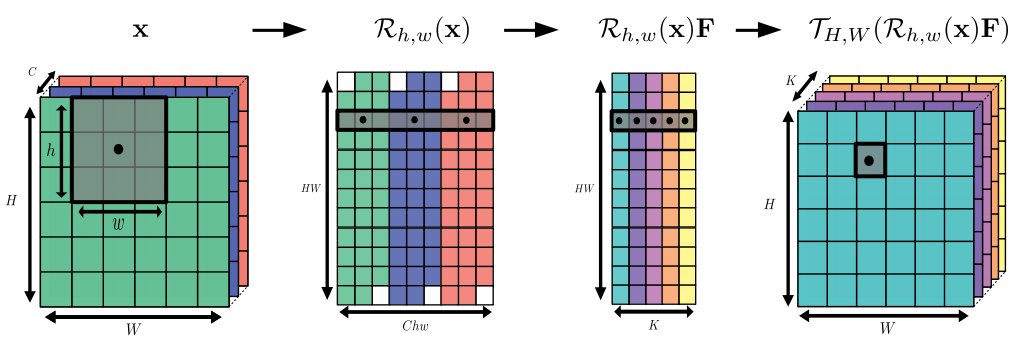
\includegraphics[width=\textwidth]{figures/reshape.png}
\caption{Depiction of the reshape operations and localy linear transformations computed in the convolutional layers. We've tried to represent the evolution of the input tensor as it goes along the convolution processing. For each drawing, the mathematical value of what it is supposed to represent is written on top of it. The scale isn't respected between steps but we've tried to bring consistency in the channels depiction. The greyed box represent the receptive field of the convolution filters at one particular coordinate. This coordinate is depicted by the black dot and can be followed along operations. The different colors represent the different channels either in the input ($C$ channels) or the output ($K$ channels) tensor. The whited squares in the second step recall the zero padding of the input.}
\label{fig:reshape}
\end{figure}

~\\

With these reshape operators, the output $\rmZ \in \R^{H \times W \times K}$ of a convolutional layer with $K$ filters is given by:

\begin{align}
\label{eq:convo_comp}
 \rmZ = \sigma(\mathcal{T}_{H, W} (\mathcal{R}_{h, w}(\rmX)~\rmF))
\end{align}
~\\
, where $\sigma$ is some non-linear activation function, $\rmF \in \R^{Chw \times K}$ is the matrix of weights describing the convolution filters and $\rmX \in \R^{H \times W \times C}$ is the output 3-D tensor of the preceding layer. The convolutional layer uses the matrix of filters $\rmF$ in order to compute localy linear transformations of its input patches defined by the reshape operator $\mathcal{R}_{h, w}$.

\section{Learning fast-transform Structures}
\label{sec:palm}
\todo[inline]{This whole section "Learning fast-transform structures" has been copy-pasted from the quick-means paper. Must modify it.}
\paragraph{Linear operators structured as products of sparse matrices.}
The popularity of some linear operators from $\R^{D}$ to $\R^{D}$ (with $D<\infty$)
 like Fourier or Hadamard transforms comes from both their mathematical 
 properties and their ability to compute the mapping of some input $\rvx\in\R^D$ with efficiency, typically in $\mathcal{O}\left (D\log D\right )$ in lieu of  
  $\mathcal{O}\left (D^2\right)$ operations.
The core feature of the related fast algorithms is that the matrix $\rmW\in\sR^{D\times D}$ of such 
linear operators can be written as the product $\rmW=\Pi_{q\in\intint{\nfactors}}\rmS_q$ 
of $\nfactors=\bigO{\log D}$ sparse 
matrices $\rmS_q$ with $\left \|\rmS_q\right \|_0=\mathcal{O}\left( D \right)$ non-zero 
coefficients per factor \cite{LeMagoarou2016Flexible,Morgenstern1975Linear}:
for any vector $\rvx\in\sR^M$, $\rmW\rvx$ can thus be computed as $\mathcal{O}\left (\log D\right )$ products $\rmS_0 \left (\rmS_1 \left (\cdots \left (\rmS_{Q-1}\rvx\right )\right )\right )$ between a sparse matrix and a vector, the cost of each product being $\bigO{D}$, amounting to a $\mathcal{O}(D \log D)$ time complexity.

\paragraph{Approximating any matrix by learning a fast transform.} When the linear operator $\rmW$ is an arbitrary matrix, one may approximate it with such a sparse-product structure by learning the factors $\left \lbrace\rmS_q\right \rbrace_{q\in\intint{Q}}$ in order to benefit from a fast algorithm.
\cite{LeMagoarou2016Flexible} proposed algorithmic strategies to learn such a factorization. Based on the proximal alternating linearized minimization (\texttt{PALM}) algorithm~\cite{bolte2014proximal}, the \texttt{PALM} for Multi-layer Sparse Approximation (\palm) algorithm aims at approximating a matrix $\rmW\in\sR^{D \times d}$ as a product of sparse matrices by solving


\begin{align}
\label{eq:palm4msa}
\min_{\left \lbrace\rmS_q\right \rbrace_{q\in\intint{Q}}} \left \|\rmU -  \prod_{q\in\intint{\nfactors}}{\rmS_q}\right \|_F^2 + \sum_{q\in\intint{\nfactors}} \delta_{\mathcal{E}_q}(\rmS_q),
\end{align}
~\\
where for each $q\in\intint{Q}$, $\delta_{\mathcal{E}_q}(\rmS_q)=0$ 
if $\rmS_q \in \mathcal{E}_q$ and $\delta_{\mathcal{E}_q}(\rmS_q)=+\infty$ otherwise. $\mathcal{E}_q$ is a constraint set that typically imposes a sparsity structure on its elements, as well as a scaling constraint. 
Although this problem is non-convex and the computation of a global optimum cannot be
ascertained, the \palm algorithm is able to find %good 
local minima with convergence guarantees. 

\todo[inline]{Fin du copy-pasta}

In~\cite{LeMagoarou2016Flexible}, the authors further propose an extension of \palm called \hpalm that rely on some hierarchical optimization strategy to get better approximation results.

% The matrix-vector multiplication $\rmW\rvx$ , e.g. a linear transformation  of the vector $\rvx \in \R^D$ by the transformation matrix $\rmW \in \R^{D\times D}$, is usually computed in time $\bigO{D^2}$. Nevertheless, some particular linear transforms such as the Hadamard transform come with a fast-algorithm that allows to reduce the computation time of their application to $\bigO{D \log D}$. Recent work~\cite{LeMagoarou2016Flexible} has pointed out that this acceleration is associated with the possible re-writting of such transformation matrix as a product of $Q=\log{D}$ sparse factors $\Pi_{q \in \intint{Q}}S_q$ with $\forall i ||S_i||_0 = \bigO{D}$. Hence, we can compute the matrix-vector multiplication right to left in time $\bigO{D \log D}$. 

\section{Contribution}

In this paper we propose to use the \hpalm algorithm on the various weights matrix of a pretrained neural network so that they all are expressed as product of sparse matrices instead of dense matrices. This simple idea would allow to drastically reduce both the space complexity of any layer in the network \textit{and} the time complexity for their computation on CPU. Indeed, even though GPU usage would definitely benefits from the space complexity saving, their highly parallelized computation wouldn't take advantage of the sparse structure of the matrices. In contrary to~\cite{yang2015deep}, these benefits wouldn't come at the cost of introducing bias on the choice of a fixed fast-transform structure for the weight matrices.

\paragraph{In convolutional layers (Equation~\eqref{eq:convo_comp})} The dense matrices of weights have $\bigO{ChwK}$ parameters. Expressing them as product of $Q = \log K$ sparse factors with each $\bigO{Chw}$ non-zero values allows to reduce this space complexity to $\bigO{Chw \log K}$, assuming $Chw~>~K$. The time complexity saving is tightly associated with this reduction of parameters: it lowers from time $\bigO{HWChwK}$ to time $\bigO{HWChw \log K}$, that is applying the fast-transform to each of the $HW$ patches.

\paragraph{In fully-connected layers (Equation~\ref{eq:fc_comp})} The dense matrices of weights have $\bigO{Dd}$ parameters. Let $A:=\max(D, d)$ and $B:=\min(D, d)$, then expressing these dense matrices as product of  $Q = \log K$ sparse factors with each $\bigO{A}$ non-zero values allows to reduce this space complexity to $\bigO{A \log B}$. The time complexity saving is once again associated to this reduction of parameters: it also lowers from $\bigO{Dd}$ to $\bigO{A \log B}$.

\section{Experiments}
\label{sec:experiments}

\subsection{Experimental setting}
\paragraph{Implementation details} Hardware (CPU frequency etc.) and Software (library, etc.) details
\paragraph{Datasets} MNIST, SVHN, CIFAR10/CIFAR100, Imagenet
\paragraph{Models} Download pretrained models from the Internet or re-train them
\paragraph{\palm algorithm settings} Sparsity level, number of factor, Hierarchical, error delta threshold, number of iteration

\subsection{Number of parameters} In the whole compressed model. Compare to other methods and show that accuracy results are not compromised by the reduction of the nbr of parameter

\subsection{Inference time} Show results on CPU. Maybe make a proof of concept on raspberry

\subsection{Carbon footprint} It would be awesome to present results of accuracy/time versus GPU and give insight on the difference in carbon footprint between CPU and GPU. Need to read about that though. Suivre la meme technique de calcul que~\cite{DBLP:journals/corr/abs-1906-02243}


\section{Conclusions}\label{sec:conclusions}
We worked hard, and achieved very little.

\bibliographystyle{abbrv}
\bibliography{palmnet}

\end{document}
This is never printed
